% iaus2esa.tex -- sample pages for Proceedings IAU Symposium document class
% (based on v1.0 cca2esam.tex)
% v1.04 released 17 May 2004 by TechBooks
%% small changes and additions made by KAvdH/IAU 4 June 2004
% Copyright (2004) International Astronomical Union

\NeedsTeXFormat{LaTeX2e}

\documentclass{iau}
\usepackage{graphicx}
\usepackage[T1]{fontenc}

\title[Everything we’d like to do with LSST data, but we don’t know (yet) how] %% give here short title %%
{Everything we'd like to do with LSST data, but we don't know (yet) how}

\author[Ivezi\'{c}, Konoli, \& Juri\'{c}]   %% give here short author list %%
{\v{Z}eljko Ivezi\'{c}$^1$, Endrju \DJ{}. Konoli$^1$ \& Mario Juri\'{c}$^1$
}

\affiliation{
$^1$ Department of Astronomy, University of Washington, \\ Box 351580, Seattle, WA 98195-1580, USA\\ 
                               email: {\tt ivezic@astro.washington.edu}
}

\pubyear{2017}
\volume{325}  %% insert here IAU Symposium No.
\pagerange{1--10}
% \date{?? and in revised form ??}
\setcounter{page}{1}
\jname{Astroinformatics}
\editors{M. Brescia, eds.}

\begin{document} 
\maketitle

\begin{abstract}
The Large Synoptic Survey Telescope (LSST), the next-generation optical imaging survey 
sited at Cerro Pachon in Chile, will provide an unprecedented database of astronomical
measurements. The LSST design, with an 8.4m (6.7m effective) primary mirror, a 9.6 sq. deg.
field of view, and a 3.2 Gigapixel camera, will allow about 10,000 sq. deg. of sky to be 
covered twice per night, every three to four nights on average, with typical 5-sigma depth 
for point sources of  $r$=24.5 (AB). With over 800 observations in $ugrizy$ bands over a 
10-year period, these data will enable a deep stack reaching $r$=27.5 (about 5 magnitudes 
deeper than SDSS) and faint time-domain astronomy. The measured properties of newly 
discovered and known astrometric and photometric transients will be publicly reported 
within 60 sec after closing the shutter. The vast database of about 30 trillion observations 
of 40 billion objects will be mined for the unexpected and used for precision experiments 
in astrophysics. In addition to a brief introduction to LSST, we discuss a number of 
astro-statistical challenges that need to be overcome to extract maximum information 
and science results from LSST dataset.  
\keywords{surveys, galaxies, stars: statistics}
\end{abstract}

\firstsection % if your document starts with a section,
                     % remove some space above using this command.


\section{Introduction \label{sec:lsst}}

The last decade has seen fascinating observational progress in optical imaging surveys.
The SDSS dataset is currently being greatly extended by the ongoing surveys such as 
Pan-STARRS (Kaiser et al. 2010) and the Dark Energy Survey (Flaugher 2008). The Large Synoptic 
Survey Telescope (LSST)  is the most ambitious survey currently planned in the visible band
(for a brief overview, see Ivezi\'{c} et al. 2008). The unparalleled LSST survey power is due to 
its large \'etendue (see Figure~\ref{fig:Gemini}). 

The goals of the LSST are driven by four main science themes: probing dark energy and dark matter, 
taking an inventory of the Solar System, exploring the transient optical sky, and mapping the 
Milky Way. The LSST will be a large, wide-field ground-based system designed to obtain multiple 
images covering the sky visible from Cerro Pach\'{o}n in Northern Chile. 
The system, with an 8.4m (6.4m effective) primary mirror, a 9.6 deg$^2$ field 
of view, and a 3.2 Gigapixel camera, will allow, on average, about 10,000 deg$^2$ of sky to be covered 
using pairs of 15-second exposures in two photometric bands every three nights, 
with a typical 5$\sigma$ depth for point sources of $r\sim24.5$. The system is designed to 
yield high image quality as well as superb astrometric and photometric accuracy \footnote{For 
detailed specifications, please see the LSST Overview Paper,
\cite{Ivezic08LSST}, and the LSST Science Requirements Document, http://ls.st/srd}. 
The survey area will cover 30,000 deg$^2$ with $\delta<+34.5^\circ$, and will be imaged multiple times in six bands, $ugrizy$, covering the wavelength range 320--1050 nm. About 90\% of the 
observing time will be devoted to a deep-wide-fast survey mode which will observe an
18,000 deg$^2$ region over 800 times (summed over all six bands) during the anticipated 
10 years of operations, and yield a coadded map to $r\sim27.5$. These data will result in 
databases including about 20 billion galaxies and a similar number of stars, and will 
serve the majority of science programs. The remaining 10\% of the observing time 
will be allocated to special programs such as a Very Deep and Fast time-domain 
survey. More details about various science programs that will be enabled by LSST data
can be found in the LSST Science Book (Abell et al. 2009) and at the LSST website (www.lsst.org). 

First light for LSST is expected at the end of  2019 with a small commissioning camera (144 Mpix), with 
the full 3.2 Gpix camera integrated in 2020. The construction phase of LSST, funded by the U.S. 
National Science Foundation and Department of Energy, started in 2015 and is progressing
according to the planned schedule (see Figure~\ref{fig:summit2019}). 

\begin{figure}[t!]
\begin{center}
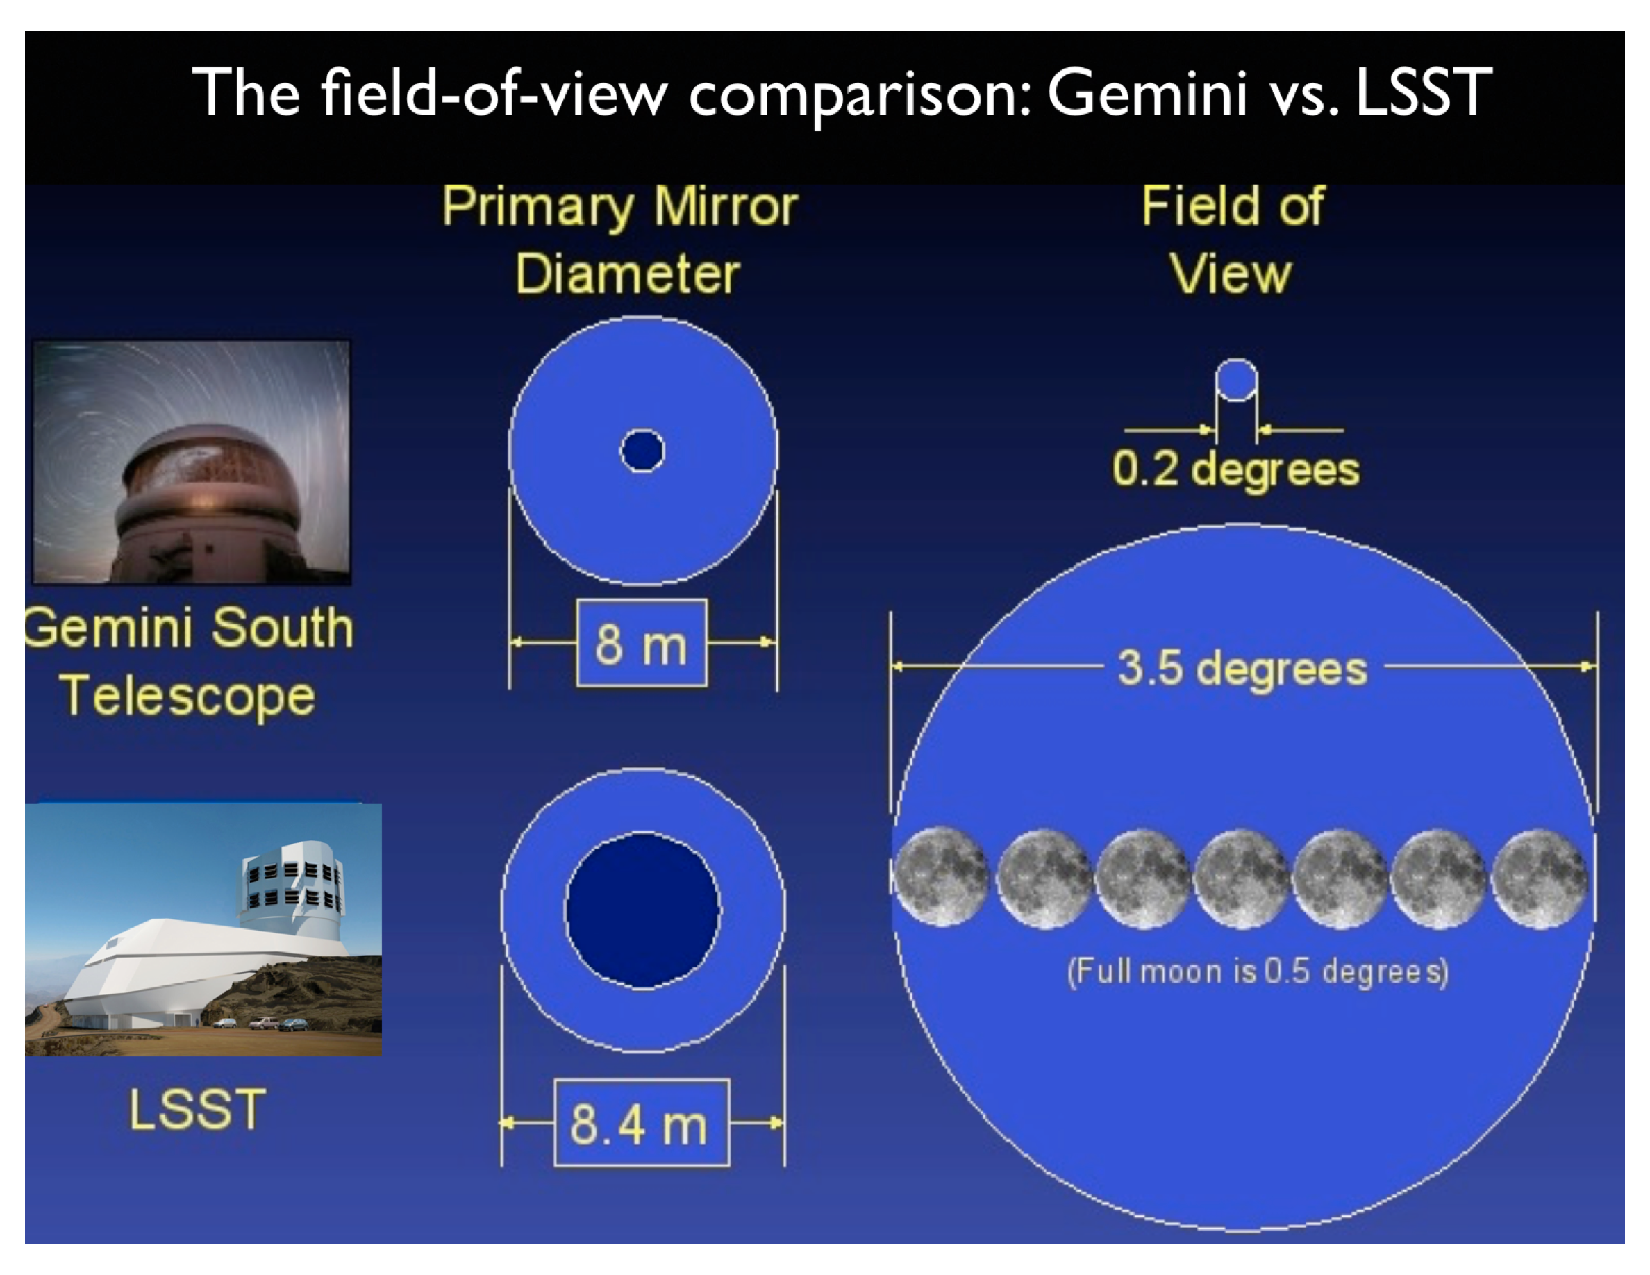
\includegraphics[width=0.99\textwidth, angle=0]{LSSTvsGemini.pdf} 
\caption{
A comparison of the primary mirror size and the field-of-view size for LSST 
and Gemini South telescopes. The product of the primary mirror size and 
the field-of-view size, the so-called \'etendue (or grasp), a characteristic 
that determines the speed at which a system can survey a given sky area 
to a given flux limit, is much larger for LSST. Figure courtesy of Chuck Claver.}
\label{fig:Gemini}
\end{center}
\end{figure}


\begin{figure}[t!]
\begin{center}
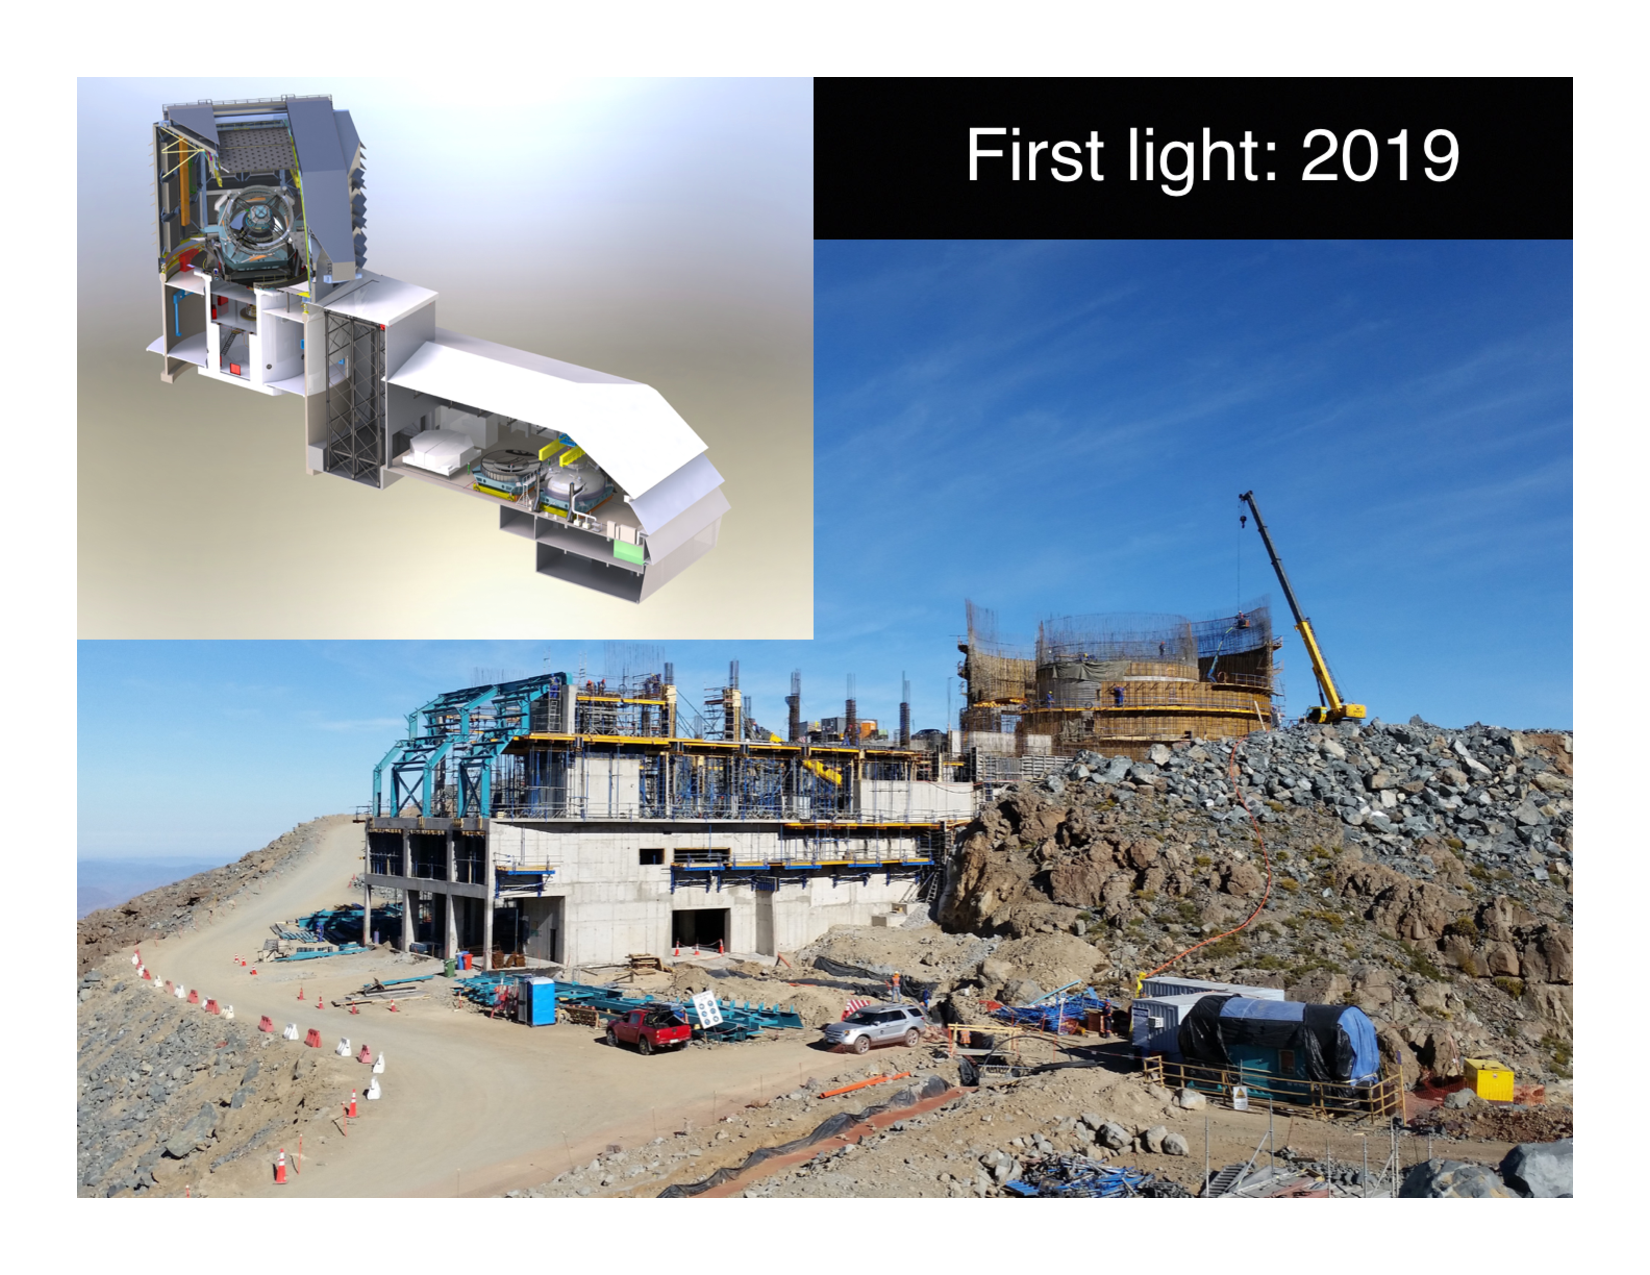
\includegraphics[width=0.99\textwidth, angle=0]{summit2019.pdf} 
\caption{
The inset in the top left corner shows a cut-away render of the LSST Observatory building. 
The rest of the figure shows a photograph of the LSST summit at the time of this 
Symposium (September 2016). First light for LSST is expected with a small engineering
camera in 2019, and with the full 3.2 Gpix camera in 2020. For more 
photographs, see https://www.lsst.org/gallery/image-gallery}
\label{fig:summit2019}
\end{center}
\end{figure}



\section{LSST Data Analysis Challenges}


The LSST project will deliver data products that will enable a large number of cutting-edge science 
programs (Juri\'{c} et al. 2016). Nevertheless, depending on the topic, the path from LSST data 
products to science results and journal papers may sometimes require additional challenging
analysis work. These challenges, representative of the era of Big Data, stem from:
\begin{itemize}
\item Large data volumes (petabytes)
\item Large numbers of objects (billions)
\item Highly multi-dimensional spaces (thousands)
\item Unknown statistical distributions 
\item Time-series data (irregular sampling)
\item Heteroscedastic errors, truncated, censored and missing data
\item Unreliable quantities (e.g. unknown systematics and random errors)\\
\end{itemize}

{\it Everything we'd like to do with LSST data, but we don’t know
  (yet) how} is a catchy title but somewhat inaccurate. First, we most
certainly do not include here ``everything'', and second, we and our
LSST colleagues already have at least some ideas for how to approach
most of problems discussed below.  We hope that this contribution will
help motivate others to join us in this thinking, and to engage in
the work needed to maximize LSST's scientific yields.\\

To begin and stimulate this conversation, we've selected selected topics where substantial
preparatory work is needed to optimally analyze data sets the size of the
LSST. These are:
\begin{enumerate}
\item The interpretation of spectral energy distributions (SEDs)
%\item Spatial correlations
\item The identification of moving objects
\item The characterization and classification of variable stars 
\item Understadning systematic measurement uncertainties
\item Characterizing astrophysical simulations and astrophysical
  systematics
\item Devising new or ehnanced algorithms to process LSST data\\
\end{enumerate}

We emphasize that many other members of LSST Science Collaborations contributed to
the formulation of this, by all means, incomplete list. In the remainder of this section, 
we discuss these topics in a bit more detail. 


\subsection{Interpretation of spectral energy distributions (SEDs)}

Efficient and robust interpretation of time-resolved multi-band photometry for “billions and 
billions” of objects is bound to yield unprecedented science results. A combination of 
required measurement precision and relatively wide bandpasses will require careful
interpretation of LSST data. 

A broad-band photometric system, such as LSST, aims to deliver calibrated in-band flux
\begin{equation}
\label{Fb}
             F_b = \int{F_\nu(\lambda) \phi_b(\lambda) d\lambda},
\end{equation}
where $F_\nu(\lambda)$ is specific flux of an object {\it at the top} of 
the atmosphere and $\phi_b(\lambda)$ is the normalized system response 
for the given band (the $\lambda^{-1}$  term reflects the fact that CCDs 
are photon-counting devices)
\begin{equation}
\label{PhiDef}
\phi_b(\lambda) = {\lambda^{-1} S_b(\lambda) \over \int{\lambda^{-1} S_b(\lambda) d\lambda}}.
\end{equation}
Here, $S_b(\lambda)$ is the overall atmosphere + system throughput
\begin{equation}
\label{SDef}
         S_b(\lambda) = S_b^{sys}(\lambda) \times S_b^{atm}(\lambda). 
\end{equation}

Numerous science programs can be cast as constraining the behavior of the SED 
$F_\nu(\lambda)$ given the measured broad-band fluxes\footnote{Traditionally, the in-band flux is 
reported on a magnitude scale, and the LSST adopted AB magnitudes defined as 
$m_b = -2.5\log_{10}\left({F_b \over 3631 \, {\rm Jy}}\right)$.}, $F_b$, and the 
normalized system response, $\phi_b(\lambda)$, with
$b=(u,g,r,i,z,y)$. Because of the integration 
over broad bandpasses, forward modeling using a trial SED (either empirical or model based) is 
typically superior to ``correcting data'' (fluxes, positions, sizes). Examples of such programs, 
where SEDs presumably depend on relevant astrophysical parameters, include, 
\begin{enumerate}
\item Photo-z algorithms: the observed galaxy and quasar SEDs depend on the redshift of an intrinsic SED  
(due to expansion of the universe, source evolution, and intergalactic extinction; see e.g. Bolzonella et al. 2000). 
\item Photometric parallax for stars, where measured colors can be used to constrain the effective
          temperature  and luminosity (e.g. Juri\'{c} et al. 2008). 
\item Photometric metallicity for stars (trained using spectroscopic metallicities, see Ivezi\'{c} et al. 2008b). 
\item Interstellar extinction along the line of sight for stars in the Milky Way disk (see, e.g., Berry et al. 2012). 
\end{enumerate}

There are number of open interesting issues that are still being worked on by the community: 
\begin{itemize}
\item What are the relative advantages and disadvantages of machine
  learning methods compared to methods based on fitting
          SED templates (both empirical and simulated). How can we
          incorporate ancillary data (and priors) within the photo-z
          methods, for example utilizing angular cross-correlation of 
         photometric and spectroscopic sample so galaxies (Newman 2008)? 
\item What are the impacts of heteroscedastic noise, priors, and truncated and censored data? 
\item How much will ``per-visit processing'' of LSST data help (due to varying bandpasses $\phi_b(\lambda)$ 
          because of the unavoidable variations in $S_b^{atm}(\lambda)$)? 
\item What is the best way to handle posterior probability density functions, how much is gained compared 
         to simple (e.g. maximum likelihood) point estimates, what are the optimal compression procedures, etc.?  
\item How should the parameter covariances be handled (the same question is also valid pretty much everywhere 
          else below)? 
\end{itemize}



% \subsection{Spatial correlations}

% For point processes, correlation functions characterize how far (and on what scales) the distribution of points 
% differs from a random distribution (see, e.g., Martinez \& Saar 2002). Correlation functions, and in particular 
% autocorrelation functions, have been used extensively throughout astrophysics with examples of their use 
% including the characterization of the fluctuations in the densities of galaxies and quasars as a function of
% luminosity, galaxy type and age of the universe. The key aspect of these statistics is that they can be used as 
% metrics for testing models of structure formation and evolution directly against data (for example, in order 
% to compare the predictions of general relativity vs. modified gravity theories to observations). In addition to 
% correlation functions, examples of the use of spatial correlations include matched-filter finders of dwarf 
% galaxies and streams/tidal tails (e.g., see Rockosi et al. 2002; Willman et al. 2005), and characterization of 
% the LMC/SMC and Virgo overdensity morphologies. 

% Some open and interesting questions include: 
% \begin{itemize}
% \item Do contemporary methods scale up to billions of points across the sky?
% \item Can this work (e.g. matched-filter search for dwarf galaxies) be done directly in database?
% \item What are the best methods for visualizing spatial correlations? 
% \end{itemize}



\subsection{Moving objects}

The catalogs generated by LSST will increase the known number of small
bodies in the Solar System by a factor of 10-100, among all
populations (Jones et al. 2015). The median number of observations for
Main Belt asteroids will be on the order of 200-300, allowing sparse
lightcurve inversion to determine rotation periods, spin axes, and
shape information. The current strawman for the LSST survey strategy
is to obtain two visits of the same field per night (each ``visit''
being a pair of back-to-back 15s exposures), separated by about 30
minutes, and covering the entire observable sky every 3-4 days
throughout the observing season.

The main reason for two observations per night is to help association of observations of the same object from 
different nights, as follows. The typical distance between two nearby asteroids on the Ecliptic, at the faint fluxes 
probed by LSST, is a few arcminutes (counts are dominated by Main Belt asteroids). Typical asteroid motion during 
several days is much larger (of the order a degree or more) and thus, without additional information, detections of individual 
objects are ''scrambled''. However, with two detections per night, the motion vector can be estimated. The motion 
vector makes the linking problem much easier because positions from one night can be approximately extrapolated 
to future (or past) nights.

There are several interesting open questions regarding moving objects: 
\begin{itemize}
\item Cadence optimization: are two visits per night really needed?
  Would perhaps a substantial increase in the computing power solve
  the association problem with just a single detection per night?
\item How robust and efficient would be a full Bayesian approach for
  characterizing the orbits of asteroids (see, e.g., Virtanen et al. 2001)? 
\item How hard is it to deploy shift-and-coadd method for KBOs and
  more distant objects on the scale of LSST?
\item What are the most robust and efficient methods for sparse lightcurve inversion of several million asteroids? 
\end{itemize}


\subsection{Variable stars}

Early in the survey, LSST will be discovering about 100,000 variable
stars per night at high Galactic latitudes (Ridgway et al. 2014), and
probably many more at low latitudes (but the forecast is less
certain). The total number of variable stars to be discovered by LSST
is of the order 100 million (the total number of detected and measured
stars will be about 20 billion). In addition, about 1000 new
supernovae are expected to be discovered every observing night. A
number of statistical questions need to be answered for the full
exploitation of this dataset:
\begin{itemize}
\item How to best distinguish regular (periodic) from irregular
  variability when the data are sampled irregularly and when the
  variability may be wavelength dependent? 
\item How to distinguish short from long variability timescales? 
\item What are the best methods for the robust detection of
  variability, and for anomaly detection?  Recent developments in
  compressed sensing, and deep learning have the potential to
  revolutionize the analysis of variability and transient
  detection. By exploiting the sparseness of the data and the models
  that might be fit to these data it maybe possible to characterize
  and classify sources in a way that is both flexible and robust to
  noise.
\item What are the best methods for characterization and
  classification of a broad range of variability (especially in case
  of sparse data early in the survey)? How do machine learning methods
  compare to light curve template-based methods?  Are there metrics that will
  enable a general classification scheme for identifying sources that
  might need follow up observations.
\item What is the impact of heteroscedastic noise, astrophysical
  priors, and truncated and censored data?
\item Can light curve and objects characterization and classification be done directly in database?  
\end{itemize}

%It is rather likely that LSST will greatly benefit from pre-cursor variability surveys, such as Gaia 
%(see, e.g., Eyer et al. 2015). 


\subsection{Systematic measurement uncertainties}

Due to large number of objects in LSST samples, many science programs, including cosmology,
will be sensitive to systematic errors. In many case the volume of the
available data will mean that systematics are the dominant source of
uncertainty. The primary drivers for the LSST measurements that could
be limited by systematics include:
\begin{enumerate}
\item ensuing that the astrometry can be measured with random and systematic errors at the miliarcsec level,
\item calibrating the photometry with random and systematic errors at the milimag level,
\item measuring galaxy shapes (cosmic shear) with the PSF known across
  the focal plane to a level where the autocorrelation of PSF
  residuals are smaller than $10^{-7}$),
\end{enumerate}
These effects will need to be quantified as functions of position on the sky, observing 
conditions (e.g. atmospheric seeing, sky brightness), and object properties
(e.g., brightness, colors, size). Some of the open questions include:
\begin{itemize}
\item How can the impact of unknown SEDs be quantified? 
\item What is the impact of atmosphere (due to variable seeing and transmissivity, 
          differential chromatic refraction and intrinsic stochasticity)? 
\item How can we robustly quantify multiplicative and additive errors in galaxy shear measurements? 
\item How can we control systematic errors in photometric redshifts? 
\item Given billions of objects measured a thousand times, how do we know that sqrt(N) will still work
          in this regime? 
\end{itemize}



\subsection{Astrophysical simulations and astrophysical systematics}

The expected precision of the LSST measurements and their resulting
constraints on cosmological and astrophysical models requires the
development of simulation and modelling tools of equal or better
precision. These tools will need to provide predictions for what the LSST
will observe (in order to define effective survey strategies for the
LSST),  interpret the observations in the context of physically
motivated models, and generate multiple realizations of a simulation
to characterize the uncertainties or covariances within the
cosmological and astrophysical constraints.

Simulations come in a number of different flavors. Instrument
simulations that model the optical performance of the LSST (e.g.\ the
impact of the atmosphere, telescope, and camera on the image quality),
cosmological simulations that model the evolution in structure within
the universe, and mock or synthetic catalogs which provide
realizations of the sky with appropriate distributions of the
astrophysical properties of sources and their uncertainties.

The scale of the required simulations range from approximations of the
technical parameters that describe the LSST (opsim; Reuter et
al. 2015), single realizations of an image from an LSST sensor (Bean
et al 2014), large scale mock catalogs of asteroids (Slater et al.\
2016), to full simulations of representative volumes of LSST data
(Bean et al 2016). Many of the required simulation tools are in
development (e.g.\ Connolly et al. 2014). There remain, however, a
number of challenges for these tools to be commonplace within the
community.

\begin{itemize}
\item How do we support the generation of large scale simulations? The
  computational resources required to generate cosmological
  simulations, and in particular series of simulations for
  characterizing the covariance of cosmological models, are large and
  could exceed the resources available to individual investigators.
\item How do we share simulations in a manner similar to the
  availability of observation data? Often the sizes of simulated data
  sets exceed those from the observational data sets and are all ready
  approaching the PB scale. Transferring the generated simulations or
  mock catalogs from supercomputing centers to where they might be
  analyzed will stress academic network capacities.
\item What is the impact of baryonic effects on dark matter halo
  profiles? The current generation of hydrodynamical simulations do
  not simulate large cosmological volumes. Approximations, where lower
  resolution or dark matter only models are used to identify regions
  of interest in the simulation that are then re-simulated at higher
  resolution, can lead to biases in any derived correlations as they
  are not representative volumes of the universe.
\item What are the main feedback mechanisms in galaxy formation and
  what is the best way to handle nonlinear galaxy bias?
\item How can we best address intrinsic alignments of galaxy shapes with the density field? 
\item How can we best extract the information about the evolution of the Milky Way galaxy using 
         LSST measurements of 20 billion stars? 
\item How can we best extract the information about the evolution of the Solar System using LSST 
         measurements of a few million asteroids?  
\end{itemize}

\subsection{LSST System Enhancements and New Algorithms}

LSST is an automated {\em facility} that will deliver not only raw images, 
but also fully reduced data products (calibrated single-epoch images,
multiple flavors of co-adds, and a variety of catalogs). Its cadence will 
be optimized to enable a balanced science return across the four key science
areas (Section~\ref{sec:lsst}). Its products have been designed to enable the
derivation of a large fraction of those results, without the need to fully
understand the details of the LSST instrument, algorithms, or to begin
from raw pixel data.

To make this possible, the LSST project is making a major investment in
computing infrastructure, software, and processing algorithms.  Yet it is
quite clear that more and better are always possible; even marginal
improvement in performance (of both hardware and software) could yield
significant additional science returns.  While {\em some} of the open issues
listed below are already being addressed by groups both within and outside
the LSST construction project, substantial further research could be done.

Again, these are simply the most obvious examples; the list is by no means complete.

\begin{itemize}
\item Observing strategy (cadence) optimization can yield improvements
  in total open-shutter time for the survey, but also can improve the
  utility of angular and temporal sampling functions and dithering
  patterns (Delgado et al. 2014). It is, therefore, important to
  develop a scheduling algorithm that can efficiently address
  potential evolution of the LSST observing system and evolution of
  its science drivers. The LSST Project will develop a scheduling algorithm
  that meets the survey requirements, but the complexity of the problem and
  the potential return on investment\footnote{e.g., just 1\% effective improvement
  in LSST scheduling is roughly equivalent to $\sim4$\$M in operational cost.}
  argues for further research.
\item LSST does not plan to deliver specialized crowded field reductions
  or catalogs; images of crowded regions of the Milky Way will be
  processed with the same code utilized elsewhere, but perhaps with
  different priors used in object detection and deblending stages (i.e., to
  a very good approximation, every object observed towards the Galactic
  center is a star). A purpose-built (multi-epoch capable) crowded field
  code capable of dealing with LSST source densities and data volumes
  would tremendously enhance the value of LSST's Galactic data set.
\item No LSST data products have been explicitly designed to enable the
  detection and characterization of diffuse (e.g., ISM) or extremely
  low-surface brightness structures (e.g., LSB galaxies recently discovered
  by projects such as Dragonfly). Developing specialized codes to enable this
  type of processing may add significant value to the data set
  collected by LSST.
\item Complex galaxy models (e.g. tidal tails of merged galaxies) will
  not be fit by standard (data release) LSST pipelines. Such a tool
  would greatly help in understanding gravitational potential around
  judiciously selected galaxies.
\item Forward modeling of images on per visit basis (termed Multifit
  in LSST Data Management context) is superior to analysis of co-added
  images (because of varying observing conditions).  A particularly
  intersting problem is one of simultaneous forward modelling of data
  from {\em different} data sets (e.g., LSST and WFIRST). While there is
  substantial ongoing development (e.g. the Tractor code, see Lang et
  al. 2016), including within LSST Project (e.g., Bosch et al., ???),
  many statistical and other issues remain open and will require
  substantial further research to find the optimal approach.
\item At the required precision level, the LSST point spread function
  (PSF) will depend on time, instrument state, source position, and
  source color (more precisely, on in-band SED shape) , see Meyers \&
  Burchat (2015). Robust and precise determination of the PSF will
  therefore be a rather non-trivial undertaking. LSST project is
  required to characterize the PSF to the degree described in the SRD,
  but further improvements may be possible.
\item Shift-and-stack algorithm, for co-adding images along arbitrary
  space-time trajectories, that could be efficiently deployed for
  large datasets would likely have a major impact on outer Solar
  System science. LSST Data Manageent system will not deliver
  shift-and-stack pipelines or data products, but these could be easily
  built on top of the open source code LSST DM will deliver.
\item Image differencing will be used to detect transient sources in
  LSST data stream (transients will be reported within 60 seconds from
  closing the shutter). In order to control the false positive rate,
  new sophisticated algorithms will have to be developed to account
  for varying observing conditions (e.g. the treatment of differential
  chromatic refraction effects due to varying airmass, and the
  color-dependent PSFs). At the same time, they will need to be fast
  enough to meet the 60 seconds processing time limit. The LSST project
  is developing these to enable its code deliverables, but broader
  research in this earea would always be welcome.
\item The SEDs of newly discovered transients will be poorly known (at least early after their discovery).
It is not clear yet what characterization and classification algorithms would be the best for separating 
the most interesting transients that require prompt followup from the background of much more numerous
transients which can be analyzed on much longer timescales without significant loss of science outcome.
\item While there are well developed methods for the classification of light curves of variable stars
(e.g. Richards et al. 2011), transient classification with sparse data is a much harder problem. 
\item Jointly processing data from LSST and other surveys (e.g., Euclid or WFIRST) would
certainly result in a superior data set than the one produced individually
by either of these great projects (for details see, e.g., Jain et al. 2015). It is not clear, however,
how exactly to implement these ideas in practice, especially given that the survey overlap will be 
significantly truncated (either by position on the sky, e.g., for WFIRST, or by brightness, e.g. for Gaia).
\item Finally, LSST data processing will be performed in the context of a
relatively traditional HPC-like computing facility utilizing proven, low-risk,
technologies (e.g., HT Condor, Pegasus). Similarly, LSST catalog data will be served
to the users by way of relational databases (albeit of advanced, distributed, kind). Research into 
alternative models of processing (e.g., making use of the public cloud or workflow 
systems like Apache Spark) or data storage and serving (e.g., no-SQL
databases, or next-generation experiments such as SciSQL) would be of great interest.
If successful, these efforts could significantly enhance the ability of the community
to perform affordable large-scale catalog computations or even {\em ab-initio}
from-pixels reprocessings.\\
\end{itemize}

A number of use cases above may be possible for the users to
run at the LSST Data Access Center. LSST has reserved approximately 10\% of
its total capacity to enable end-user analyses and generation of added value
data products.

Furthermore, many of the use cases would be best tackled by enhancing
existing LSST pipelines or building completely new functionality on top of
the one already provided by LSST. All of the source code for the LSST
pipelines will be publically available, enabling these kinds of endeavors.

Finally, LSST Operations have been built with the assumption that, in
addition to the work within the facility, the community will make new
discoveries and breakthroughs in areas of algorithms and data products.
Such enhancements, developed by the community, can be incorporated into
standard LSST processing becoming a part of the official LSST alert
streams and/or data releases.

\section{Discussion}

Due to size and complexity of LSST dataset, and susceptibility of many
of its major science goals to systematics in both measured quantities
and astrophysical predictions, substantial preparatory work is
required to fully exploit LSST dataset. The bottleneck for science
will not be data availability but instead our ability to extract
useful and reliable information from data.

Here we have summarized some of the most obvious research directions
required to enhance LSST science outcome. The main anticipated work
areas include:
\begin{itemize}
\item advanced astronomical digital image processing,
\item statistical modeling and analysis,
\item data mining and machine learning,
\item high performance computing,
\item astrophysical simulations, and
\item multi-dimensional and temporal data visualization.  
\end{itemize}

LSST data analysis and astro-informatics \& astro-statistics fields will be closely
intertwined. This synergy will open numerous opportunities for people with "Big Data” skills.
Prospective LSST science users, across all disciplines, should collaborate and
coordinate. By working jointly we can make the LSST great% again\\
, and maximize the tremendous potential and science return of its data set.

% (XXX perhaps mention LSST Data Science Fellowship Program and astroML?). 

\vskip 0.2in 
{\it Acknowledgements}  

This material is based upon work supported in part by the National Science Foundation through
Cooperative Agreement 1258333 managed by the Association of Universities for Research in Astronomy
(AURA), and the Department of Energy under Contract No. DE-AC02-76SF00515 with the SLAC National
Accelerator Laboratory. Additional LSST funding comes from private donations, grants to universities,
and in-kind support from LSSTC Institutional Members.

\begin{thebibliography}{}
\bibitem[()]{} Berry, M., Ivezi\'c, \v Z., Sesar, B., et al.~2012, Astrophysical Journal, 757, 166

\bibitem[()]{} Bolzonella, M., Miralles, J.~M. \& Pell\'{o}, R. 2000, Astronomy \& Astrophysics, 363, 476

\bibitem[()]{} Connolly, A.J., Angeli, G.Z., Chandrasekharan, S., et al. 2014, Proceedings of the SPIE, 
          Volume 9150, id. 915014

\bibitem[()]{} Delgado, F., Saha, A., Chandrasekharan, S., et al. 2014, Proceedings of the SPIE, Volume 9150, 
          id. 915015

\bibitem[()]{} Eyer, L., Evans, D.W., Mowlavi, N., et al. 2015, \textit{{\rm ArXiv:}1502.03830}

\bibitem[Flaugher (2008)]{Flaugher08}
{Flaugher, B. 2008}, In \textit{A Decade of Dark Energy: Spring Symposium, Proceedings of
  the conferences held May 5-8, 2008 in Baltimore, Maryland. (USA). Ed. by N. Pirzkal \& H. Ferguson.}

\bibitem[Ivezi{\'c} \etal\ (2008a)]{Ivezic08LSST} {Ivezi{\'c}, {\v Z}., Tyson, J.A., Acosta, E., et al. 2008a}, \textit{{\rm ArXiv:}0805.2366}

\bibitem[()]{} Ivezi\'c, \v Z., Sesar, B., Juri\'{c}, M., et al.~2008b, Astrophysical Journal, 684, 287

\bibitem[()]{} Jain, B., Spergel, D., Bean, R., et al. 2015, \textit{{\rm ArXiv:}1501.07897}

\bibitem[()]{} Jones, R.L., Juri\'{c}, M. \& Ivezi\'c, \v Z. 2015, \textit{{\rm ArXiv:}1511.03199}

\bibitem[()]{} Juri\'{c}, M., Ivezi\'c, \v Z., Brooks, A., et al.~2008, Astrophysical Journal, 673, 864

\bibitem[()]{} Juri\'{c}, M., Kantor, J., Lim, K-T., et al. 2015, \textit{{\rm ArXiv:}1512.07914}

\bibitem[Kaiser \etal\ (2010)]{Kaiser2010}
{Kaiser, N., Burgett, W., Chambers, K., et al. 2010}, 
\textit{Proc. SPIE 7733, Ground-based and Airborne Telescopes III}, vol. 7733, 77330E

\bibitem[()]{} Lang D., Hogg, D. W. \& Mykytyn D. 2016, Astrophysics Source Code Library (ascl:1604.008)

\bibitem[SciBook]{SciBook}
{LSST Science Collaboration 2009}, 
LSST Science Book, http://www.lsst.org/lsst/SciBook, arXiv:0912.0201

\bibitem[()]{} Martinez, V. \& Saar E. 2002, Statistics of the Galaxy Distribution. Chapman and Hall/CRC.

\bibitem[()]{} Meyers, J.E. \& Burchat, P.R. 2015, Astrophysical Journal, 807, 182 

\bibitem[()]{} Reyes, R., Mandelbaum, R., Seljak, U., et al. 2010, Nature, 464, 256 

\bibitem[()]{} Richards, J.W., Starr, D.L., Butler, N.R., et al. 2011, Astrophysical Journal, 733, 10 

\bibitem[()]{} Ridgway, S.T., Matheson, T., Mighell, K.J., Olsen, K.A. \& Howell, S.B. 2014, Astrophysical Journal, 796, 53

\bibitem[()]{} Rockosi, C.M., Odenkirchen, M., Grebel, E.K., et al. 2002, Astronomical Journal, 124, 349

\bibitem[()]{} Virtanen, J., Muinonen, K. \& Bowell, E. 2001, Icarus, 154, 412

\bibitem[()]{} Willman, B., Dalcanton, J.J. \& Martinez-Delgado, D. 2005, Astrophysical Journal, 626, 85

\end{thebibliography}
\end{document}

